\section{Methodology}

\subsection{Algorithms}

In the existing studies of online social networks scalability, we found researchers have developed various partition algorithms to preserve the data locality while reducing the overhead. In this project, we decide to leverage the four graph partition algorithms, namely, random partitioning, METIS graph partitioning, community detection algorithm, and SPAR to test the partition performance in the case where different number of server is available.

The social network which needs to be partition can be represented by node and edges, where one node specifies one active user in the network, and the edge, which can be directed or indirected, stands for the existence of relationship between two connected nodes.


\subsubsection{Random Partition}

As the name suggests, random partition algorithm will cluster all the node in a random manner. The possibility for a user node to be stored in a particular server is equal to the possibility for it to be stored in another ones. Since there is no optimisation involved in the algorithm, we expected that it will have the highest overhead among all algorithm. Therefore, it can server as the baseline for our experiment.  

Another reason for choosing this algorithm is that, since we are focusing on small business with relatively small number of server available, some of the advanced techniques may not function well. Using the random partition algorithm in this situation may reduce the the effort in implementation while achieves similar performance with those advanced algorithm. Even for some large corporation such as Facebook, random partition is widely used for simplicity.

\subsection{Community Detection}

Community detection algorithm bases on the assumption that the input network involves the community structure \cite{Girvan2002} which can be detected and used as the criteria to perform the partition. The community structure is a network whose nodes can be easily divided into groups/communities, in which nodes are densely connected to each other. Whereas the inter-connection between nodes from different group is relatively sparse compared to the intra-connection of nodes within the group.

\begin{figure}[t]
  \centering
  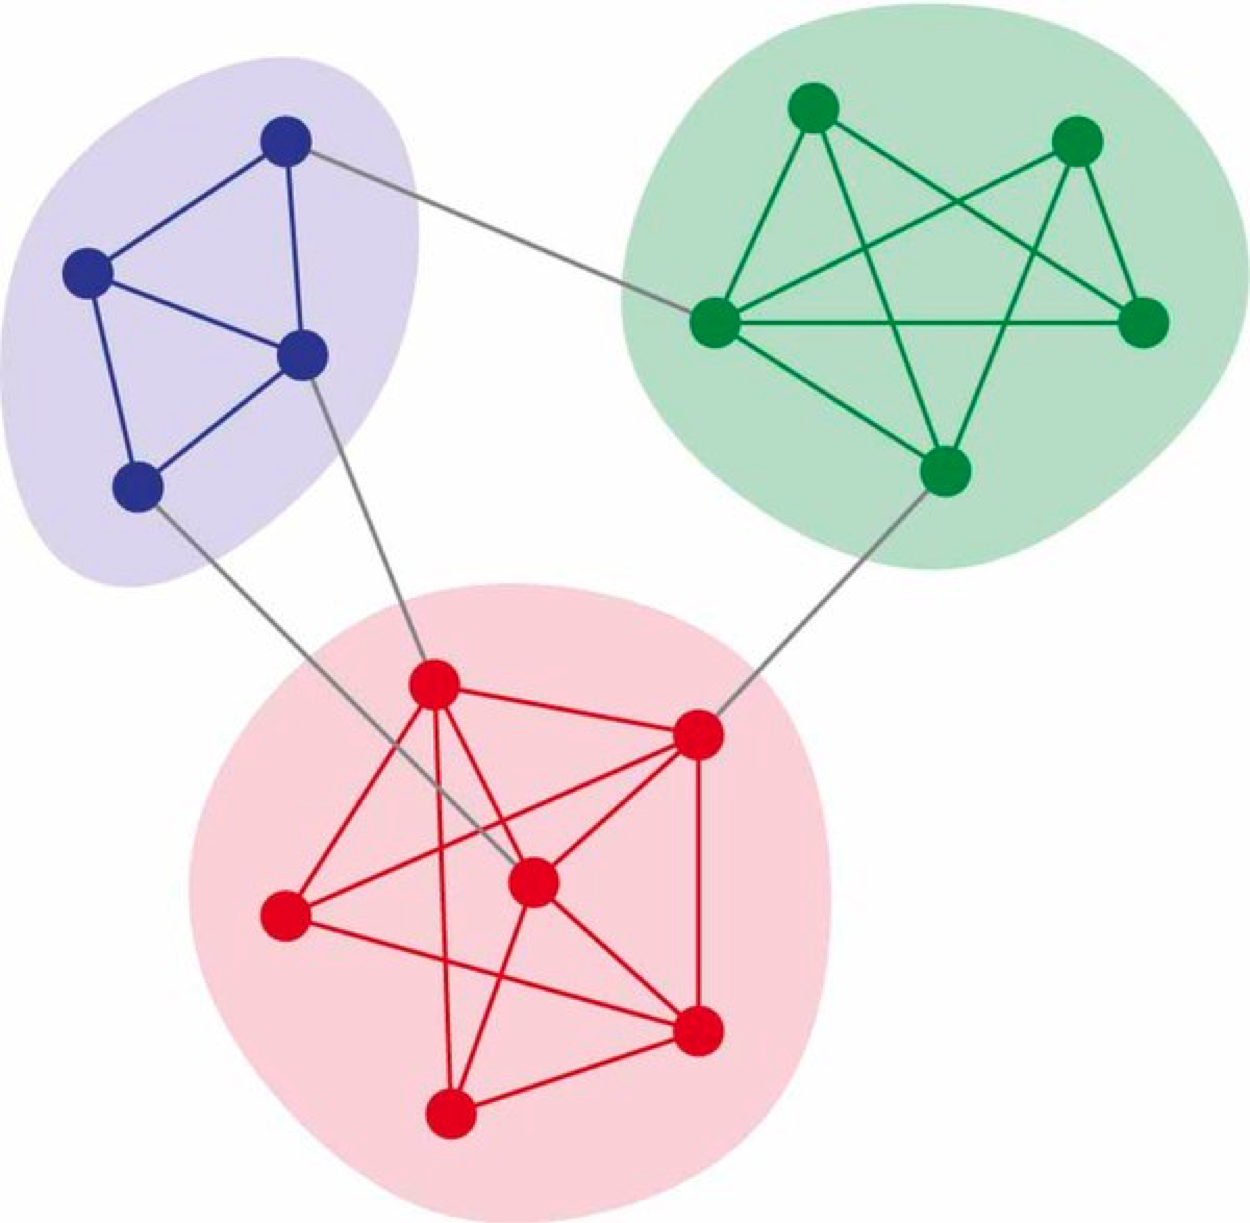
\includegraphics[width=0.5\columnwidth]{cd.png}
  \caption{Community Structure Network}\label{fig:cd}
\end{figure}


Figure \ref{fig:cd} has depicted a typical community structure network with three groups. The community detection algorithm tries to identify the structural information in the network and leverage the group information to partition the node. More specifically, take Vincent's approach as an example \cite{blondel2008fuc}, it first assigns all individual node to a different community. Then, it iteratively remove the node in its community and assigns it to other communities. It calculates the gain of all the assignment, then keeps the one with maximum gain and discards others. The iteration continues until no more assignment can be made; and the community partition reaches its local maximum. In the second phase, it build a new graph where the community of original graph become a node. The edge weight is the sum of the weight of the links between nodes in the corresponding two communities. Then it iteratively performs the algorithm to produce a hierarchical community structure in the graph. The pseudocode for the algorithm is summarised in Algorithm 1.

\begin{algorithm}
\caption{Community Detection Algorithm: Vincent's Approach}\label{euclid}
\begin{algorithmic}[1]

\Procedure{Init}{}
\ForEach {$Node \; i \in Graph$}
\State $i \gets community \; C_{i}$
\EndFor
\EndProcedure

\Procedure{Phase1}{}
\State \emph{loop}:
\ForEach {$Node \; i \in Graph$}
\State $Remove  \; i \;from \;its \;Community$
\ForEach {$Community \; c \in Graph$}
\State $Add \;i \;to \;c$
\State $Calculate \;and \;store \;gain$
\State $Remove \;i \;in \;c$
\EndFor
\State $gain \gets Max(gain)$
\State $i \gets c \; with \;gain$
\EndFor
\EndProcedure

\Procedure{Phase2}{}
\ForEach {$Community \; c \in Graph$}
\State $Convert \;c \;to \;node$
\State $edge \;weight \gets \;Sum(number \;of \;connections)$
\EndFor
\State \textbf{goto} \emph{loop}.
\EndProcedure
\end{algorithmic}
\end{algorithm}

There are various approaches to identify the communities in the network. Each of them has its own advantages in some circumstances. According to Andrea \cite{DBLP:conf/valuetools/FortunatoL09}, among various community detection algorithm, Infomap \cite{Rosvall2008} has the best performance over the others. In this experiment, we have chosen \cite{blondel2008fuc} to do the testing.


\subsection{METIS}

METIS is a multilevel graph partitioning algorithm \cite{DBLP:journals/siamsc/KarypisK98}, which consists several stages to partition a large graph. First, it tries to reduce the size of the group by collapsing the nodes and edges. Two similar nodes are grouped together and be represented by a coarser mesh. The coarser mesh then serves as a new large node with weighted edges specify the number of connection between the two meshes. After that, the process is repeated until the graph is small enough for later processing (usually less than $3$k $\sim 5$k nodes). Since the graph is small, METIS then performs a high-cost but high-quality spectral partitioning algorithm on the graph. After the partitioning, a refinement or un-coarsening phase is applied to the graph to retrieve the node back from the mesh recursively. By using the Kernighan-Lin heuristic algorithm \cite{kernighan_graph-partitioning1970}, METIS can construct back the original graph with an accurate graph partitioning solution.

\begin{figure}[t]
  \centering
  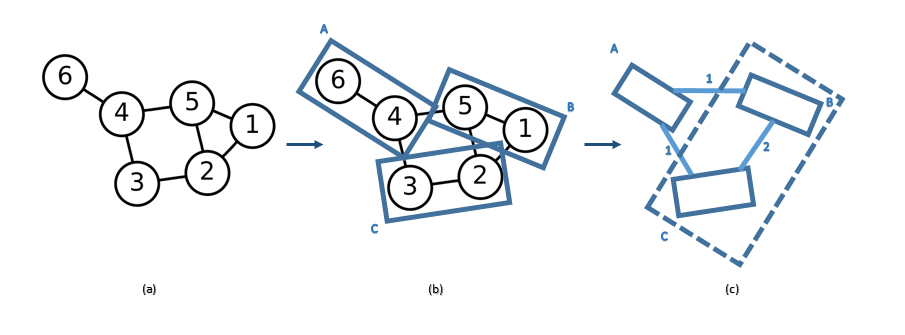
\includegraphics[width=0.95\columnwidth]{Capture.png}
  \caption{METIS Graph Reduce Algorithm}\label{fig:Capture}
\end{figure}

Figure \ref{fig:Capture} has given the basic steps of METIS. With the original graph shown in 2(a), METIS will group two nodes together to form a mesh. Figure 2(b) shows the grouped nodes represented by three meshes A,B, and C. Then, METIS treats the meshes as new nodes and repeats the process to group those large nodes. The criteria for group the node is based on the similarity of the two node. In this example, the similarity is proportion to the edge weight between two nodes. In Figure 2(c), a mesh, indicated in dash line, has formed, since the weight between mesh B and C is large than others. In this algorithm, each time the number of node/mesh is reduced by half. Unlike the community detection algorithm, which considers node context globally, METIS only groups the node/mesh based on local information such as the connection weight between neighbour. Therefore, it can merge the graph much faster than the previous methods. After the graph is reduced to small size, METIS will partition the graph and reverse the procedure to get individual node with accurate partitioning assigned.


\subsubsection{SPAR}

SPAR (Social Partitioning and Replication) is a dynamic graph partitioning algorithm, which guarantees data locality by adding or removing nodes and edges at run time \cite{DBLP:journals/ton/PujolESYLCR12}. It makes a balance between the random partition algorithm which costs a lot when it reads the user profile and the full replication algorithm which require more writing operation to the server. SPAR only performs the replication/deletion when a change of the network takes place. In other words, SPAR regards the user's’ action as heuristics to help to build up the node partition layout in the server.

In our experiment, since we use only one replication for every data, whereas SPAR dynamically creates replicas for nodes neighbour in different server, we excluded this method in the experiment. However, the algorithm itself has a good performance and may become a choice for the small companies.